\documentclass[11pt,hyperref={pdfpagemode=FullScreen}]{beamer}

\usetheme{Warsaw}

\usepackage{hyperref}
\usepackage{graphicx}
\usepackage{setspace}
\usepackage{colortbl}



\title[Join us now and share the software you'll be free]{introduction to free software\\switch to free software}
%\author{Ismail 	MTAALLAH -- 4InfoB3}
\author{Akira Treize}
%\institute{ESPRIT}
\institute{ESPRIT Libre}
%\date{8 January 2012}



\begin{document}

%diapo 0
\begin{frame}
 \titlepage
\begin{center}
% 
\includegraphics[wdith=1cm,height=2cm]{moi}
\end{center}

\end{frame}

\begin{frame} 
	\begin{center}{\Large Plan }\end{center}
	\tableofcontents[hideallsubsections]
\end{frame}
% Faire apparaître un sommaire avant chaque section
\AtBeginSection[]{
   \begin{frame}
   \begin{center}{\Large Plan }\end{center}
   %%% affiche en début de chaque section, les noms de sections et
   %%% noms de sous-sections de la section en cours.
   \tableofcontents[currentsection,hideothersubsections]
   \end{frame} 
}

%diapo 1
\section{What's the free software ?}
\begin{frame}
\frametitle{What is a free software?}


\pause \begin{block}{freedom 0}
 Freedom \alert{to run} the program, for any purpose.
\end{block}

\pause \begin{block}{freedom 1}
 Freedom \alert{to study} how the program works, and change it \alert {to make} it do what you wish
\end{block}

\pause \begin{block}{freedom 2}
  Freedom \alert {to redistribute} copies so you can help your neighbor.
 \end{block}

\pause \begin{block}{freedom 3}
Freedom \alert {to distribute} copies of your modified versions to others. 
\end{block}


\end{frame}

%diapo
\subsection{The Father of Free Software}
\begin{frame}{The Father Of Free Software}
\begin{columns}
 \begin{column}{0.5\textwidth}
  \begin{tabular}{c}
 Richard Matthew Stallman (rms)\\

\includegraphics[ height=3cm]{gnu-head}\\
GNU(Gnu is Not Unix)\\
FSF(Free Software Fundation)\\
\end{tabular} 

 \end{column}
 \begin{column}{0.5\textwidth}
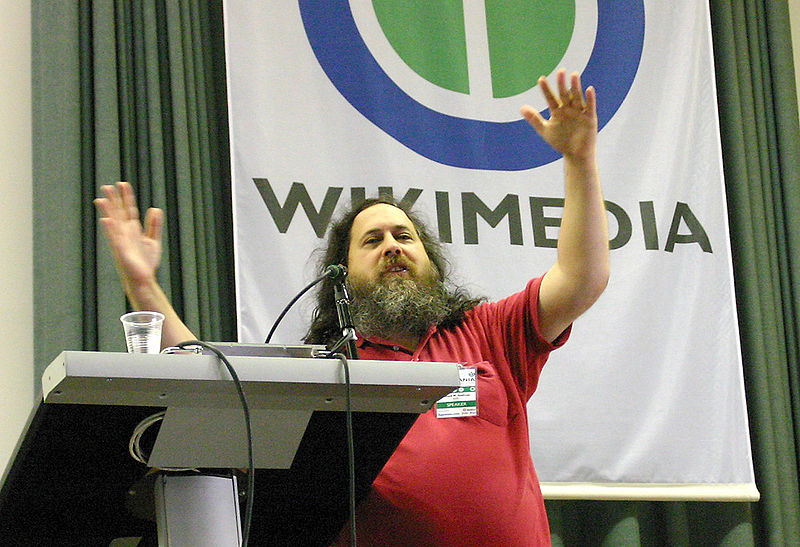
\includegraphics[width=7cm, height=7cm]{rms}
 \end{column}

\end{columns}

 
\end{frame}


%diapo 2
\begin{frame}{Free forever ?}


\begin{block}{The freedom of some must not restrict the freedom of others}
 humain  (labor law, civil law, etc...)
 What is free must remain
\newline The author retains its right in the work
\end{block}
 

\end{frame}

%frame
\begin{frame}{Other face of philosophy of free}
The philosophy of the Free now affects other areas:\newline
 \begin{itemize}
  \pause \item art (music, books, pictures) with Creative Commons licenses,
  \pause \item sharing knowledge with the collaborative Wikipedia encylopedie,
  \pause \item scientific publications,
  \pause \item different technical and recipes,
  \pause \item etc...

 \end{itemize}

\end{frame}



%diapo 
\subsection{Open source VS Free Software}
\begin{frame}
\begin{columns}
 \begin{column}{0.7\textwidth}
\onslide<1->  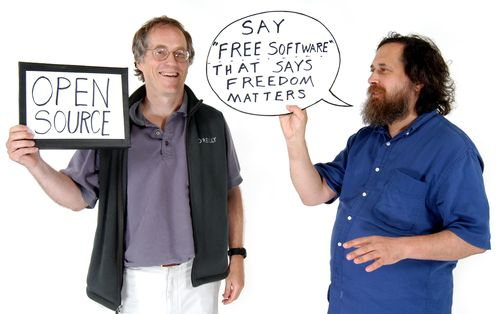
\includegraphics[width=7cm,height=7cm]{1}
 \end{column}
 \begin{column}{0.3\textwidth}
\begin{center}
\onslide<2-> OPEN SOURCE\newline
\onslide<3->\alert{!=} \newline 
\onslide<4->FREE SOFTWARE\newline
\end{center}         
               
 \end{column}

\end{columns}
\end{frame}

%diapo 4
\subsection{The various licenses:}
\begin{frame}{The various licenses:}
\begin{center}
 \begin{tabular}{|l|c|c|c|}
\cline{2-4}
\multicolumn{1}{c|}{}  &to use &to copy &to modify \\ \hline    
 Proprietary software  &\cellcolor{yellow}&\cellcolor{red}&\cellcolor{red}\\ \hline 
 Shareware             &\cellcolor{green}&\cellcolor{red} &\cellcolor{red}\\ \hline 
 Freeware              &\cellcolor{green}&\cellcolor{green}&\cellcolor{red}\\ \hline 
 Free software         & \cellcolor{green}&\cellcolor{green}&  \cellcolor{green}\\ \hline
 
  \end{tabular}
\end{center} 
\end{frame}

\section{Notion of community}
%diapo 5
\subsection{Communitys}
\begin{frame}{Community}
\begin{itemize}
 \pause \item \alert{Interactions} between users (support, advice,...)\newline
 \pause \item \alert{Interactions} between users and developers (bug,reports,suggestion features,documentation, translation)
\end{itemize}


\end{frame}

%diapo 6
\subsection{Who can develop the free software}
\begin{frame}{Who can develop the free software?}
\begin{itemize}
 \item volunteers
\begin{itemize}
 \item [-]students
 \item [-]IT in his free time 
 \item [-]anyone (why not you?)
\end{itemize}
\item employees
\begin{itemize}
 \item [-]research laboratory
 \item [-]company
\end{itemize}
\item In finally, you have hundreds of thousands of contributors
\end{itemize}
\end{frame}


\subsection{Different communities}
%diapo 8
\begin{frame}{Different communities}
\begin{columns}
 
\begin{column}{0.6\textwidth}
\begin{itemize}
 \item \alert{Global level:}  (FSF, Fondation Mozilla, KDE/Gnome, linux,..),
 \item \alert{National level:} (Ubuntu-tn, Mozilla-tn,fedora-tn,....),
 \item \alert{ESPRIT level:} (ESPRIT Libre), 
\end{itemize}
\end{column}

\begin{column}{0.4\textwidth}
\begin{tabular}{c c}
 
\includegraphics[width=1.5cm,height=2cm]{utn} & 
\includegraphics[width=2cm,height=1cm]{fsf}\\
 
\includegraphics[width=2cm,height=3cm]{mtn} &
\includegraphics[width=2cm,height=3cm]{final}\\
\end{tabular} 
  
\end{column}


\end{columns}

 
\end{frame}
%//////////////////////////////////////////////////////////////////////////////////////////////////////////////
%diapo 9
\section{Some Examples of free Softwares}
%diapo 9-1
\subsection{Firefox}
\begin{frame}
\frametitle{Firefox for Windows 7}
\begin{center}
 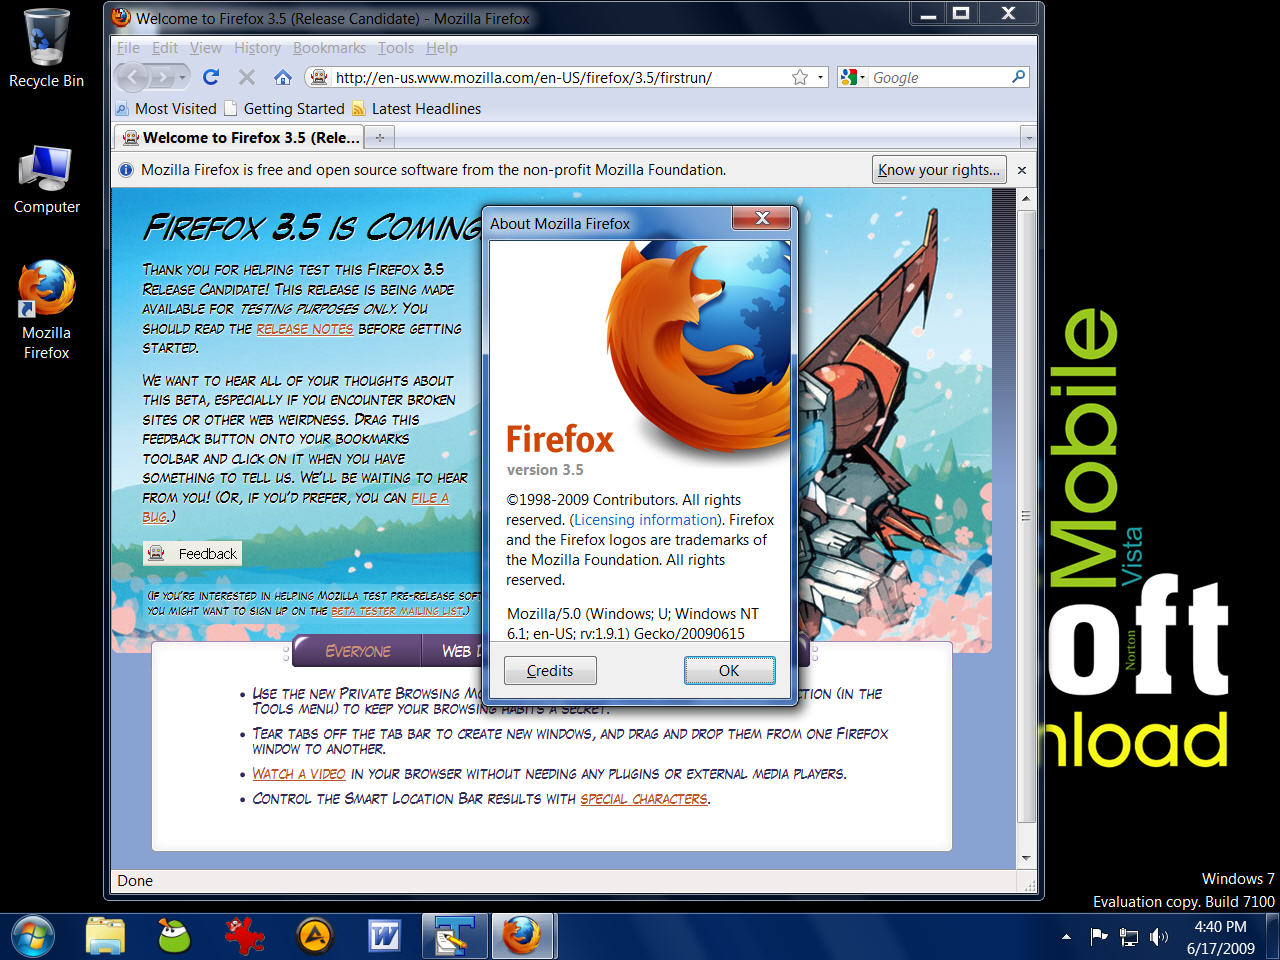
\includegraphics[width=10cm, height=7cm]{./firefox.jpg}
\end{center}
\end{frame}

%diapo 9-2
\subsection{Thunderbird}
\begin{frame}{Thunderbird for Windows}
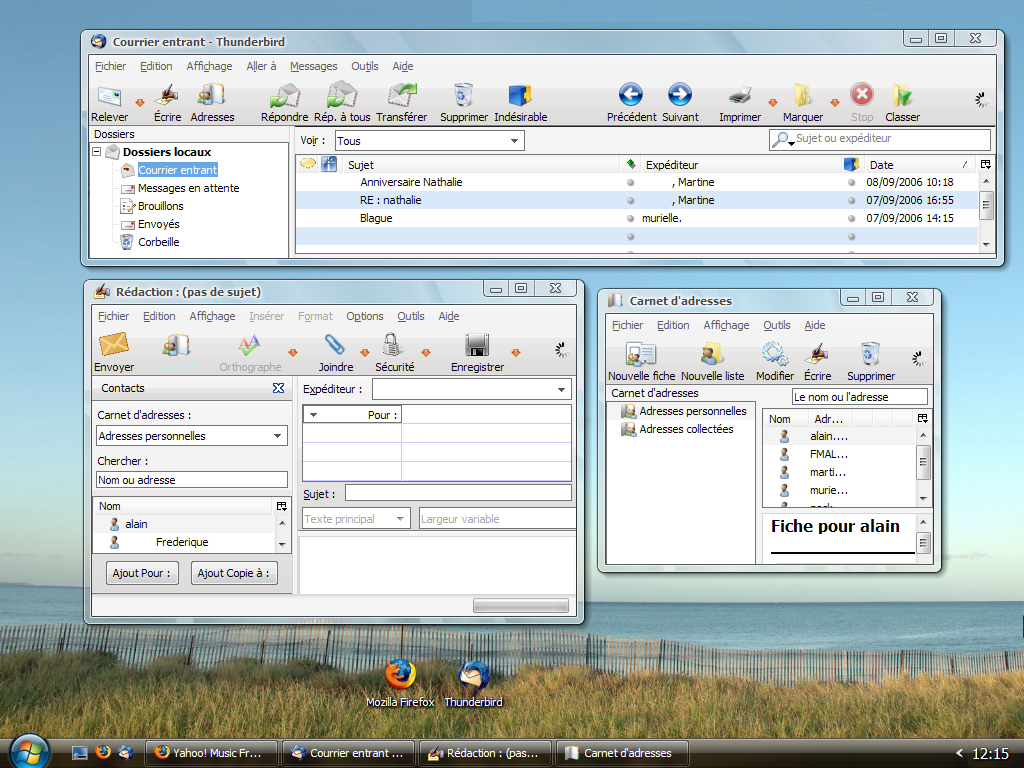
\includegraphics[width=10cm, height=7cm]{./thunderbird} 
\end{frame}

%diapo 9-3
\subsection{Gimp}
\begin{frame}{Gimp on Mac OS}
\begin{columns}
\begin{column}{0.7\textwidth}
 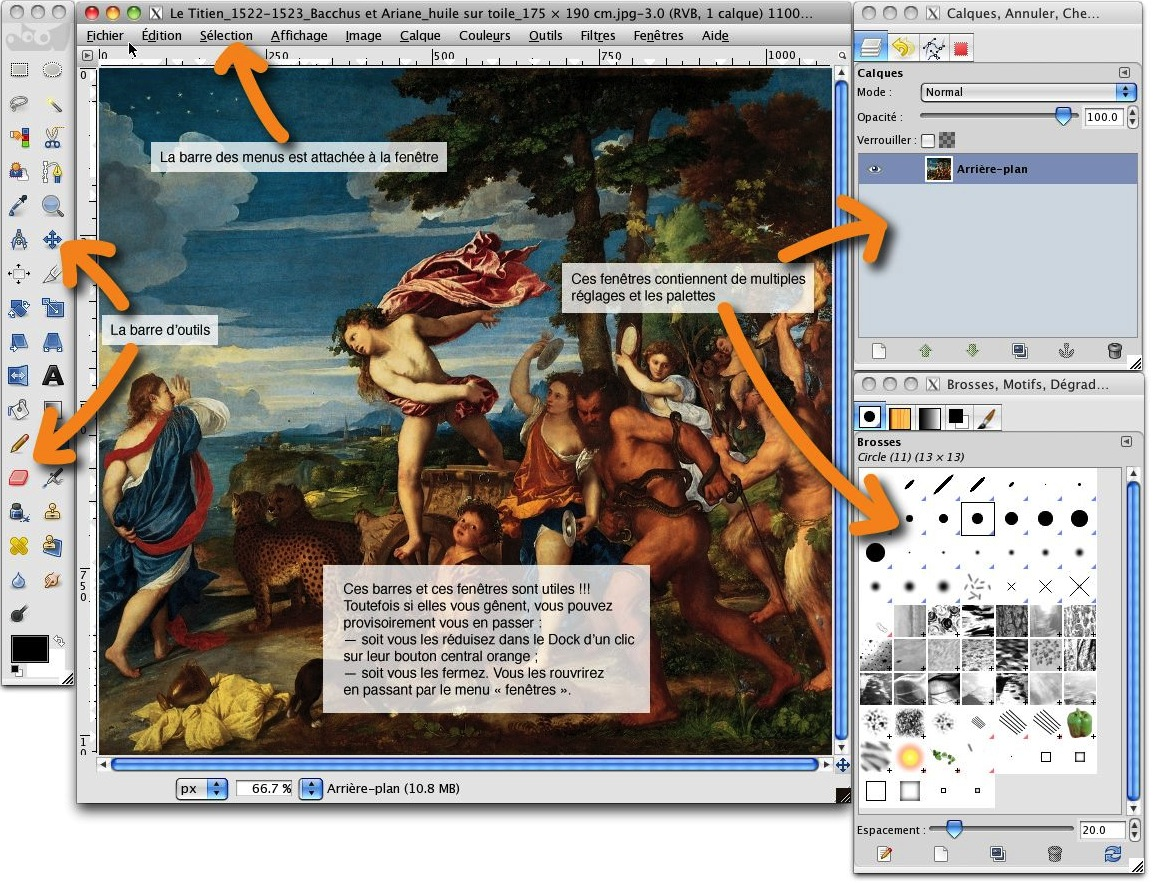
\includegraphics[width=7.5cm, height=7cm]{gimp}
\end{column}
\begin{column}{0.3\textwidth}
 \begin{center}\textbf{Gimp}\end{center}
\begin{center}GNU Image Manipulation Program\end{center}
\begin{center}
 \href {http://www.gimp.org}{\beamergotobutton{http://www.gimp.org}}
\end{center}
\begin{center}

  
\includegraphics[width=2cm, height=1.5cm]{logogimp.jpg}
\end{center}
\end{column}

\end{columns}
\end{frame}
%diapo 9-4
\subsection{Wikipedia}
\begin{frame}{Wikipedia}
\begin{columns}

\begin{column}{0.40\textwidth}
\includegraphics<1->[with=2.5cm, height=3cm]{wikipedia}
\end{column}
\begin{column}{0.6\textwidth}

\begin{itemize}

\pause \item A free, collaborative encyclopedia \newline
\pause \item Probably the most exciting free project

\end{itemize}

\end{column}
\end{columns}

\end{frame} 

%diapo 10
\section{Conclusion}
\begin{frame}{conclusion}
\begin{columns}
\begin{column}{0.7\textwidth}
The transition to free software should be step by step:
\begin{itemize}
 \item[step1:] keep your current system with using free software
 \item[step2:] coexist a free operate system same \alert {GNU/Linux} with your current system
 \item[step3:] you probably will replace your current system with \alert {GNU/Linux}
\end{itemize}

\end{column}
\begin{column}{0.3\textwidth}
 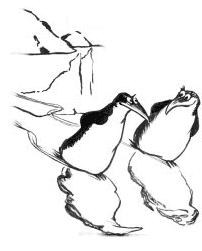
\includegraphics[with=5cm, height=3cm]{conclusion}
\begin{alertblock}{}
 The way is open but the road is long!
\end{alertblock}

\end{column}

\end{columns} 
\end{frame}



\end{document}